\chapter{ESP32 Code Architecture Overview}

This chapter explains the internal architecture of the \texttt{ESP32\_BT\_Controller} repository based on the diagram at the final of this chapter.
It describes how the Android application communicates with the ESP32 firmware, how input commands are decoded,
and how those commands become real hardware outputs (motors, PWM signals, switches), with optional telemetry and debug features.

\section{High-Level Architecture (Android App \texorpdfstring{$\leftrightarrow$}{<->} ESP32)}

The system is built around a \textbf{Bluetooth SPP (Serial Port Profile)} link:

\begin{itemize}
    \item The \textbf{Android App} sends two kinds of packets:
    \begin{itemize}
        \item \textbf{RC State packets} (continuous control state: sticks, knobs, switch bitmask).
        \item \textbf{Event packets} (button press events that trigger short pulses).
    \end{itemize}
    \item The \textbf{ESP32 firmware} receives these packets, updates shared data structures, and continuously applies the
    latest control state to the hardware outputs.
    \item Optionally, the ESP32 sends \textbf{telemetry packets} back to the Android app (panel/indicator/plot data and a one-time configuration message).
\end{itemize}

\section{Initialization Layer (Diagram: \textit{Initialization})}

At startup, \texttt{ESP32\_BT\_Controller.ino} runs \texttt{setup()}, which calls \texttt{systemInit()}.
This startup sequence prepares communications and hardware.

\subsection{Serial Initialization (\texttt{serialInit()})}
The firmware starts the USB serial port at \texttt{115200} baud.
This is mainly used for developer diagnostics (debug prints), and does not directly affect Bluetooth control.

\subsection{Bluetooth Initialization (\texttt{bluetoothInit()})}
Bluetooth SPP is initialized with:
\begin{itemize}
    \item \texttt{SerialBT.begin("ESP32-BT")}
\end{itemize}
This creates the device name the app pairs to and connects with.

\subsection{Hardware Initialization (\texttt{hardwareInit()})}
The hardware setup is divided into modules to keep the project maintainable:

\begin{itemize}
    \item \texttt{boardInit()} --- board-level setup (GPIO modes, board defaults).
    \item \texttt{i2cBusInit()} --- prepares the I\textsuperscript{2}C bus (if used).
    \item \texttt{halOutputsInit()} --- prepares PWM output channels (LEDC) and output pins.
    \item Optional: \texttt{mcpInit()} --- initializes an MCP23017 I/O expander if enabled.
    \item Optional: \texttt{i2cSensorsInit()} --- initializes external sensors on I\textsuperscript{2}C if enabled.
\end{itemize}

\section{Runtime Layer (Diagram: \textit{Runtime / main loop})}

After initialization, the Arduino \texttt{loop()} function runs continuously.
In this repository:
\begin{itemize}
    \item \texttt{loop()} calls \texttt{systemLoop()} (core control processing).
    \item \texttt{loop()} also calls \texttt{pulseUpdate()} for momentary outputs.
\end{itemize}

Inside \texttt{systemLoop()}, the main runtime pipeline is:

\begin{enumerate}
    \item \textbf{Receive and decode Bluetooth commands} (\texttt{handleBluetooth()}).
    \item \textbf{Send telemetry if due} (\texttt{sendTelemetryIfDue()}), only when an app is connected.
    \item \textbf{Apply control outputs} (\texttt{controlUpdate()}).
    \item \textbf{Optional debug printing} (gated by \texttt{debug\_config.h}).
\end{enumerate}

\section{Bluetooth Receive Subsystem (Diagram: \textit{Bluetooth RX (receiver)})}

The Bluetooth receiver module (\texttt{receiver.cpp}) is responsible for handling the raw byte stream.
Because Bluetooth data can arrive fragmented or back-to-back, the receiver uses a \textbf{rolling buffer} approach:

\begin{itemize}
    \item Read bytes from \texttt{SerialBT}.
    \item Search for valid packet headers.
    \item Wait until the full packet length is present.
    \item Copy the packet into a shared packet structure.
\end{itemize}

\subsection{Input Packets}
The repository defines fixed packet formats in \texttt{packets.h}:

\begin{description}
    \item[RC State packet (\texttt{RcPacket})] A continuous snapshot of control values (sticks, knobs, switches).
    This is the primary input for motor/servo/PWM control.
    \item[Event packet (\texttt{EventPacket})] A short packet containing an \texttt{eventId}.
    When received, the firmware triggers an event handler to generate a pulse action.
\end{description}

\section{Shared Data Model (Diagram: \textit{packets.h})}

The file \texttt{packets.h} is the central definition of all message formats used in the system.
It is important architecturally because it acts as the shared contract between modules:

\begin{itemize}
    \item The receiver writes the newest decoded state/event into global packet instances.
    \item The control layer reads those packet instances each loop.
    \item The telemetry layer creates outgoing packets using fixed layouts and checksums.
\end{itemize}

This separation makes the system easier to extend: adding a telemetry field or a new packet type is done centrally.

\section{Control Layer (Diagram: \textit{Control layer})}

The control layer (\texttt{control.cpp}) converts the latest received RC state into hardware actions:

\begin{itemize}
    \item Reads stick/knob/switch values from the current state packet.
    \item Maps control ranges into PWM ranges.
    \item Calls HAL output functions such as:
    \begin{itemize}
        \item steering PWM output,
        \item motor speed and direction,
        \item camera pan PWM,
        \item LED brightness,
        \item buzzer intensity,
        \item switch outputs.
    \end{itemize}
\end{itemize}

\subsection{Event Handling}
When an \texttt{EventPacket} arrives, the receiver triggers \texttt{controlHandleEvent(eventId)}.
This event handler maps an \texttt{eventId} to a short pulse action (for example: pulse a specific switch output).

\section{Hardware Abstraction Layer (Diagram: \textit{HAL outputs})}

The HAL output module (\texttt{hal\_output.cpp}) is responsible for the low-level hardware operations:

\begin{itemize}
    \item PWM generation using ESP32 LEDC for servos, motors, LED brightness, and buzzer intensity.
    \item Motor direction control using dedicated GPIO direction pins.
    \item Motor ramping using a timer interrupt to smooth acceleration/deceleration.
    \item Switch outputs driven either:
    \begin{itemize}
        \item directly by ESP32 GPIO pins, or
        \item via the optional MCP23017 expander.
    \end{itemize}
\end{itemize}

\section{Optional GPIO Expansion (Diagram: \textit{MCP23017 (optional)})}

If enabled, the MCP23017 provides extra I/O lines over I\textsuperscript{2}C.
The module \texttt{mcp\_io.cpp} handles:

\begin{itemize}
    \item Writing to MCP registers to control outputs.
    \item Reading inputs from MCP Port A (commonly used for indicators).
    \item Writing outputs on MCP Port B (commonly used for switches/events).
\end{itemize}

\section{Telemetry Subsystem (Diagram: \textit{Telemetry TX} and \textit{Telemetry sources})}

The telemetry subsystem (\texttt{telemetry.cpp}) sends data back to the Android app, but only when a client is connected
(\texttt{SerialBT.hasClient()}).

\subsection{Connection-Aware Behavior}
\begin{itemize}
    \item If no phone is connected, telemetry does nothing and resets its ``config sent'' state.
    \item When a phone connects, the ESP32 first sends a one-time \textbf{configuration telemetry message}
    (labels for plots/panels/indicators) so the app can populate its UI.
    \item After that, it periodically sends telemetry packets according to timing intervals.
\end{itemize}

\subsection{Telemetry Sources}
Telemetry values are produced by separate source functions (shown as \textit{Telemetry sources} in the diagram),
for example ADC readings, digital masks, and optional sensor values.
The telemetry module focuses on packet building and scheduling, not on deciding how raw data is collected.

\section{Debug Subsystem (Diagram: \textit{Debug})}

The debug subsystem (\texttt{debug.cpp}) only formats and prints information to \texttt{Serial}.
It is controlled by compile-time flags in \texttt{debug\_config.h}:

\begin{itemize}
    \item stick prints, knob prints, switch prints, and event prints can be enabled/disabled.
    \item debug does not implement Bluetooth logic or memory buffering; it is intentionally separated.
\end{itemize}

\section{Pulse Subsystem (Diagram: \textit{Pulse outputs})}

Some user actions are momentary (a button press should create a short pulse).
This repository handles that behavior in the pulse subsystem:

\begin{itemize}
    \item \texttt{pulseUpdate()} is called in the Arduino \texttt{loop()}.
\end{itemize}

This keeps ``pulse timing'' separate from the main control update and prevents outputs from staying ON unintentionally.

\section{Summary: Why the Architecture is Structured This Way}
The repository is organized as a pipeline of specialized modules:

\begin{itemize}
    \item \textbf{Receiver} isolates Bluetooth byte-stream decoding.
    \item \textbf{Packets} defines the shared communication contract.
    \item \textbf{Control} maps app inputs into actions.
    \item \textbf{HAL} performs hardware-specific output writes.
    \item \textbf{Telemetry} handles scheduling and output reporting.
    \item \textbf{Debug} provides visibility without contaminating logic code.
\end{itemize}

This separation makes the firmware easier to maintain and extend (new outputs, new telemetry fields, new sensors),
while keeping the Android app communication stable.


%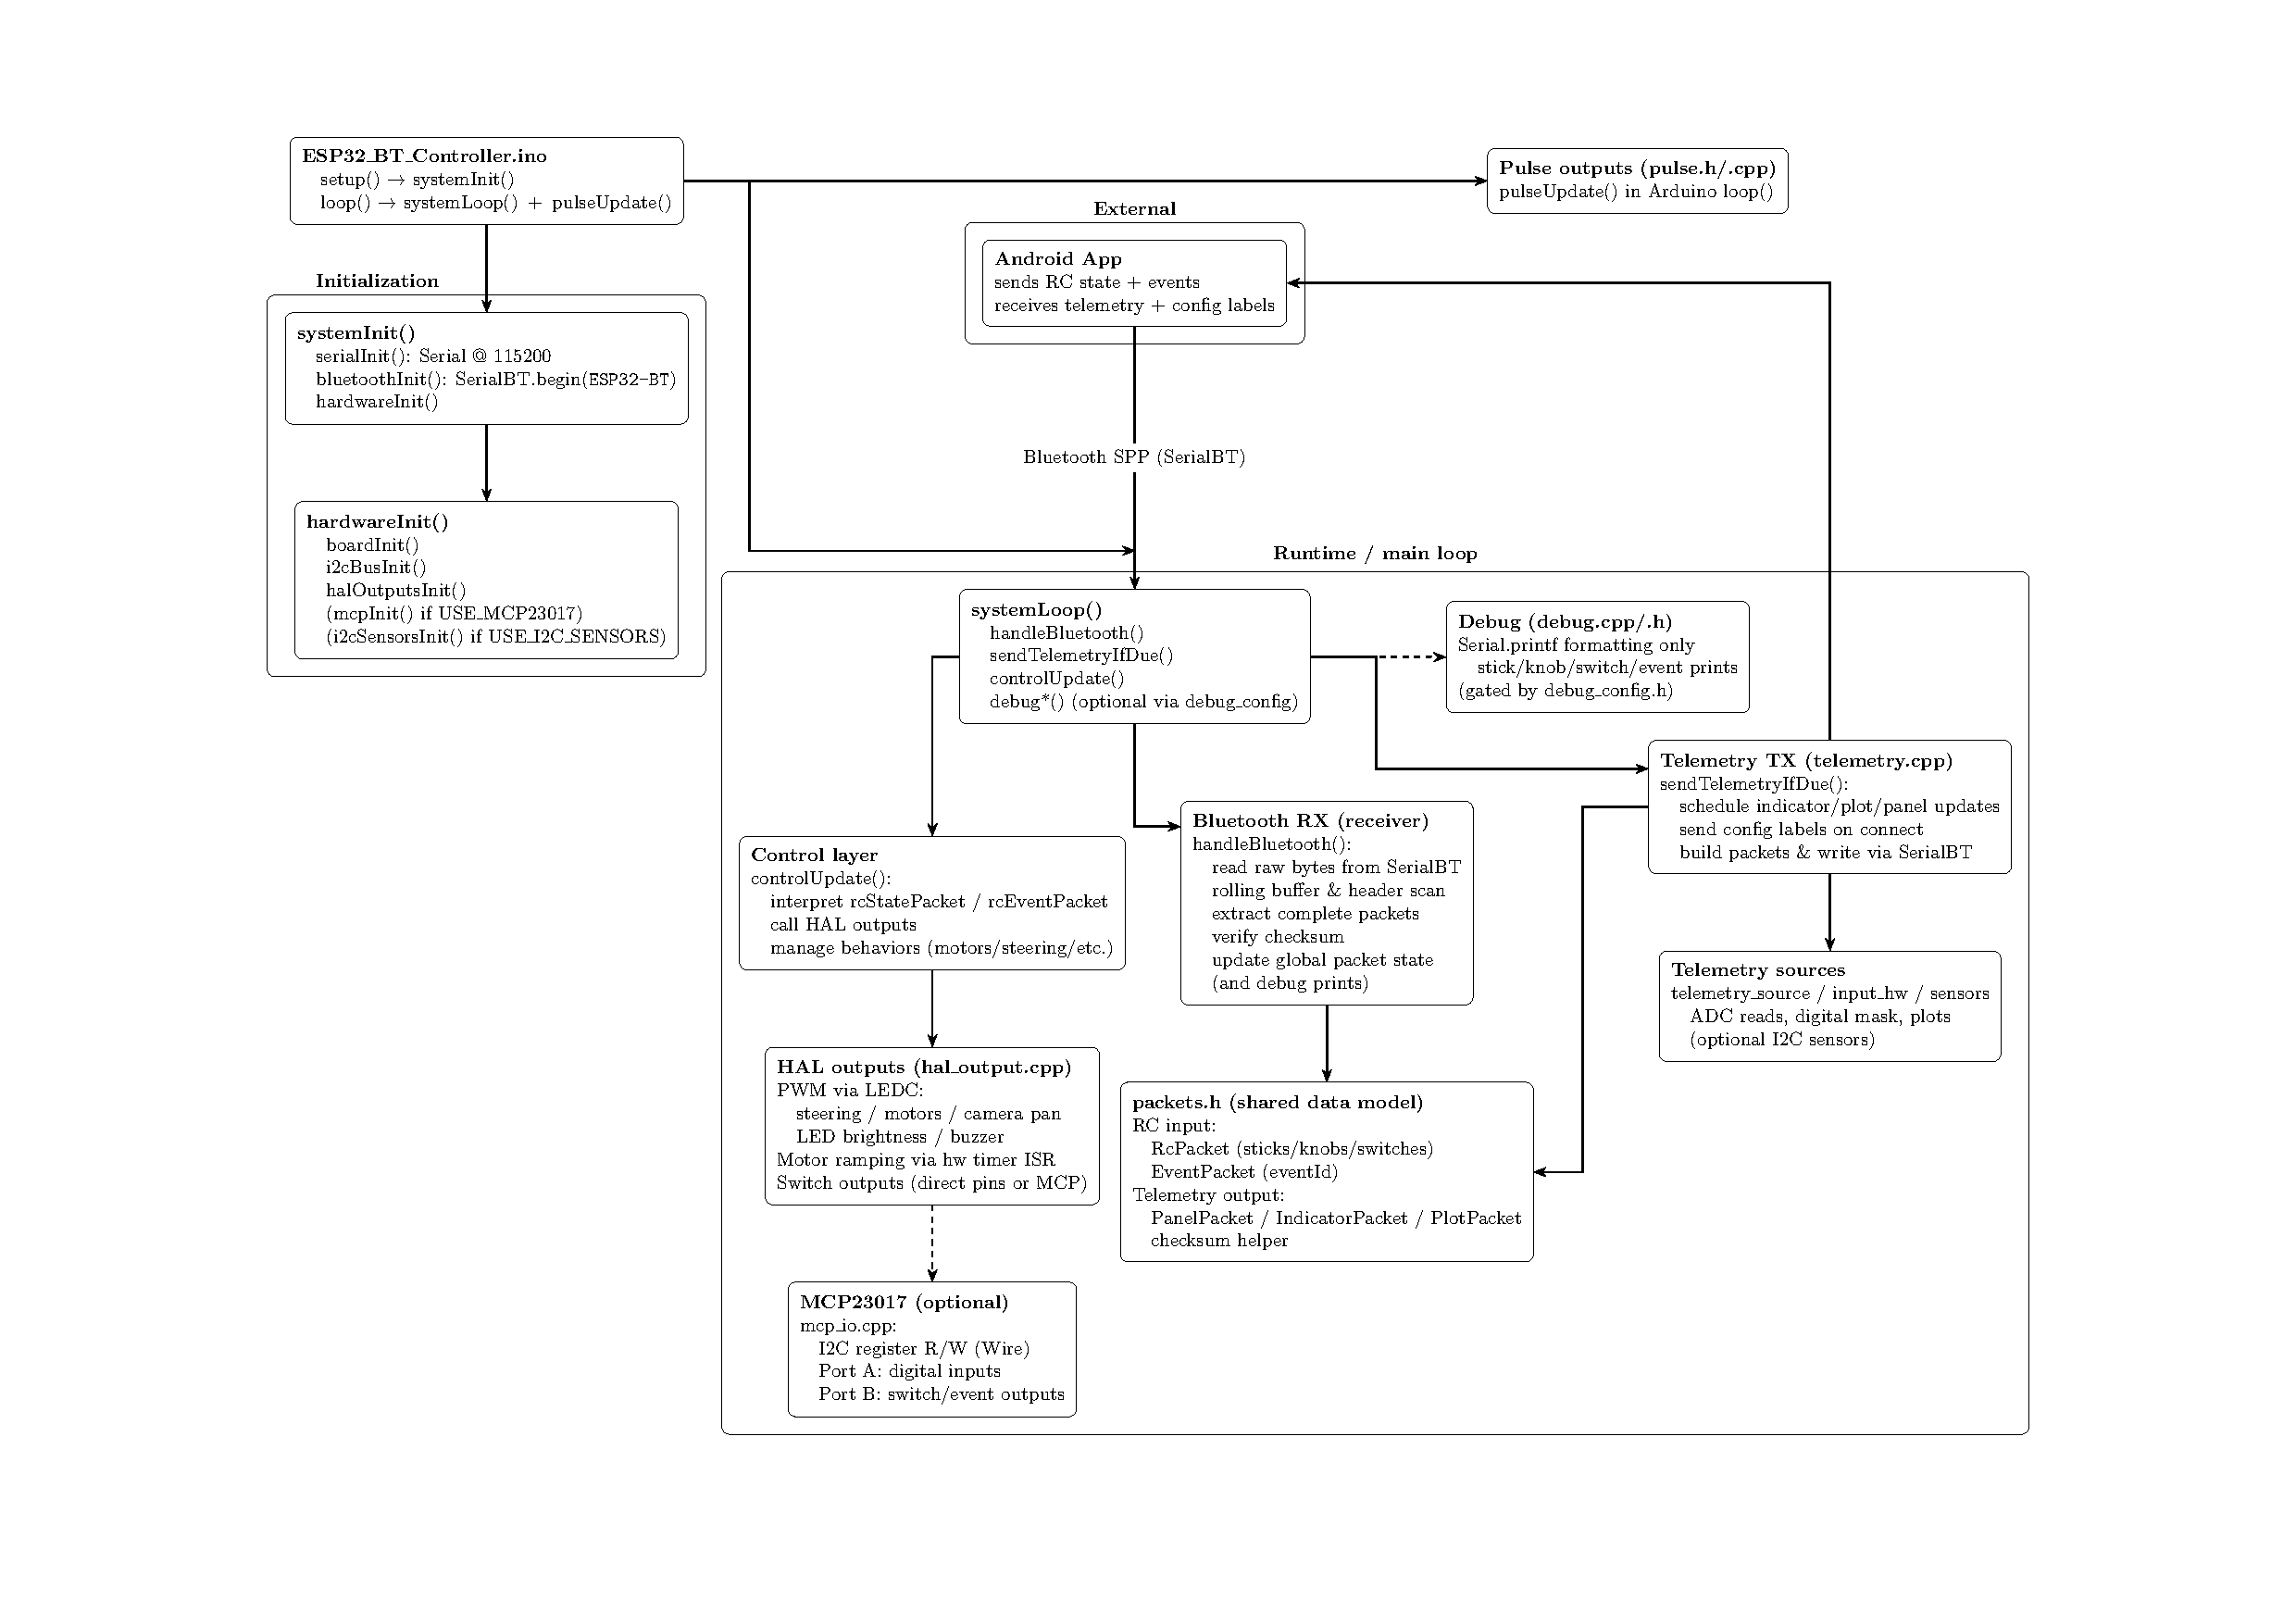
\includepdf[
%pages=1,
%landscape,
%fitpaper=false,
%pagecommand={
%    \thispagestyle{plain}
%    \begin{center}
%        \vspace*{\fill}
%        \rotatebox{90}{
%            \parbox{0.7\textheight}{
%                \centering
%                \captionof{figure}{ESP32's software architecture.}
%                \label{fig:esp32-arch}
%            }
%        }
%    \end{center}
%}
%]{Architecture_ESP32.pdf}




\includepdf[
pages=1,
landscape,
fitpaper=false,
offset=0 1cm,   % ← MOVE UP
pagecommand={
    \thispagestyle{plain}
    \begin{figure}[!b]
        \centering
        \caption{ESP32's software architecture.}
        \label{fig:esp32-arch}
    \end{figure}
}
]{Architecture_ESP32.pdf}



%\begin{landscape}
%    \begin{center}
%        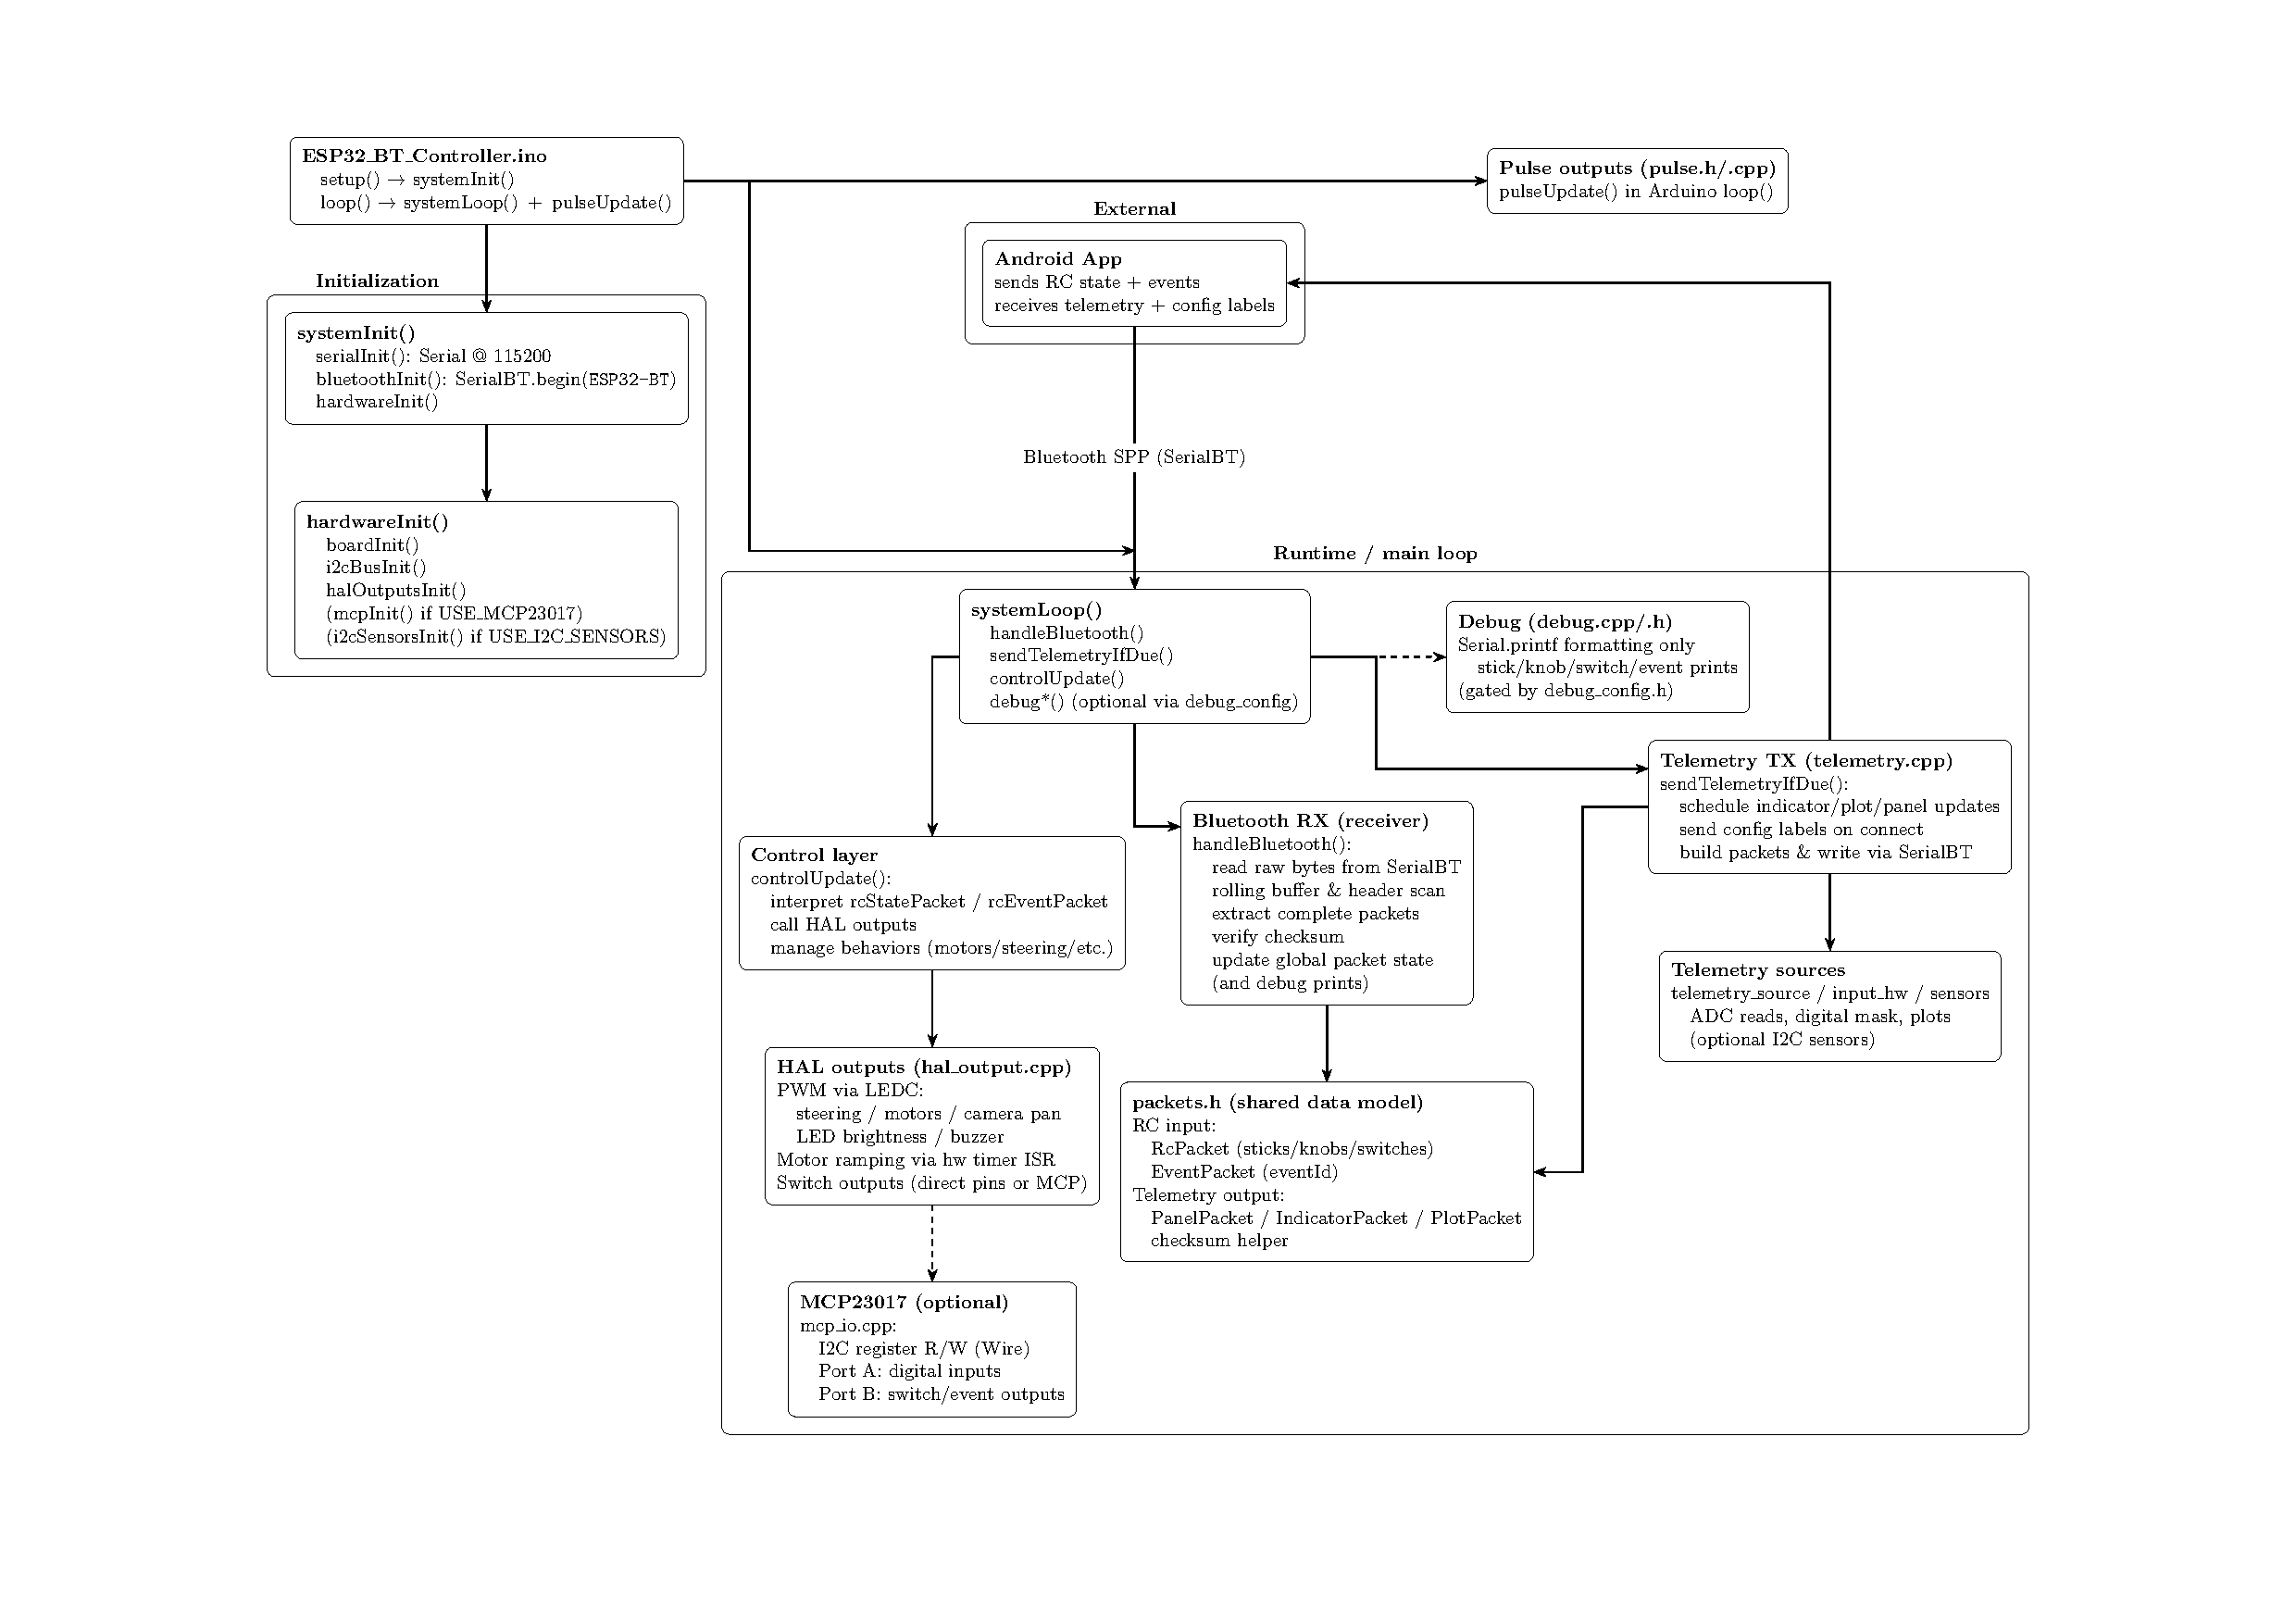
\includepdf[
%        pages=1,
%        landscape,
%        fitpaper=false]{Architecture_ESP32.pdf}
%    \end{center}
%\end{landscape}